% !TEX program = pdflatex
% =====================================================================
%  Econ Department Retreat — AI in our teaching — Emily's block (~35 min)
%  Thursday, August 27, 2026, 1:00–2:30 (Emily 1:00–1:45, Erkmen 1:45–2:30)
%  Derived from Webinar_Jun2026/teaching_webinar_FULL.tex (June 17 deck).
%  Structure:
%    0. Title + plan
%    A. The basics, quickly (3 slides, ~7 min)
%    1. Where it fits in teaching prep (5 slides, ~10 min)  [NEW — from Jul 21 notes]
%    2. Grading + student data, UVM edition (8 slides, ~15 min)
%    3. Where this could go for us + handoff (2 slides, ~3 min)
%    Appendix: FERPA backup for Q&A
%  Cut candidates if running long are marked %% CUT-CANDIDATE
% =====================================================================
\documentclass[aspectratio=169, 10pt]{beamer}

%% ============================================================
%% PACKAGES
%% ============================================================
\usepackage[T1]{fontenc}
\usepackage{lmodern}
\usepackage{graphicx}
\usepackage{booktabs}
\usepackage{array}
\usepackage{tabularx}
\usepackage{colortbl}
\usepackage{tikz}
\usetikzlibrary{positioning, calc, arrows.meta, shapes.geometric, fit, shadows}
\usepackage[most]{tcolorbox}
\usepackage{fontawesome5}
\usepackage{hyperref}
\usepackage{multicol}
\usepackage{xcolor}
\usepackage{textcomp}
\usepackage{pifont}

\graphicspath{{../Webinar_Jun2026/figures/}{figures/}}

%% ============================================================
%% COLOR DEFINITIONS
%% ============================================================
\definecolor{UVMGreen}{HTML}{154734}
\definecolor{UVMGold}{HTML}{D4A84B}
\definecolor{SlateTeal}{HTML}{1B4D5C}
\definecolor{DeepCharcoal}{HTML}{2C3E50}
\definecolor{SoftCoral}{HTML}{C0534D}
\definecolor{CoolGray}{HTML}{8899A6}
\definecolor{PaleSage}{HTML}{EDF2F0}
\definecolor{LightGold}{HTML}{FDF6E3}
\definecolor{DarkSlate}{HTML}{0F2B36}
\definecolor{AccentBlue}{HTML}{3498DB}
\definecolor{GoGreen}{HTML}{2E7D52}

%% ============================================================
%% BEAMER THEME SETUP
%% ============================================================
\setbeamercolor{structure}{fg=SlateTeal}
\setbeamercolor{normal text}{fg=DeepCharcoal}
\setbeamercolor{frametitle}{fg=SlateTeal}
\setbeamercolor{title}{fg=SlateTeal}
\setbeamercolor{subtitle}{fg=UVMGold}
\setbeamercolor{author}{fg=DeepCharcoal}
\setbeamercolor{date}{fg=CoolGray}
\setbeamercolor{institute}{fg=CoolGray}
\setbeamercolor{footline}{fg=CoolGray}
\setbeamercolor{block title}{fg=white, bg=SlateTeal}
\setbeamercolor{block body}{bg=PaleSage}
\setbeamercolor{alerted text}{fg=SoftCoral}
\setbeamercolor{item}{fg=SlateTeal}
\setbeamercolor{subitem}{fg=CoolGray}

\setbeamerfont{title}{size=\Large, series=\bfseries}
\setbeamerfont{subtitle}{size=\normalsize}
\setbeamerfont{frametitle}{size=\large, series=\bfseries}
\setbeamerfont{footline}{size=\tiny}

\setbeamertemplate{navigation symbols}{}

\setbeamertemplate{frametitle}{%
  \vskip14pt%
  \nointerlineskip%
  {\usebeamerfont{frametitle}\usebeamercolor[fg]{frametitle}\insertframetitle\par}%
  \vskip2pt%
  {\color{UVMGold}\rule{\textwidth}{1.2pt}}%
  \vskip3pt%
}

\setbeamertemplate{footline}{%
  \begin{beamercolorbox}[wd=\paperwidth, ht=16pt, right, rightskip=1.5cm]{footline}%
    \usebeamerfont{footline}\insertframenumber\,/\,\inserttotalframenumber\vskip3pt%
  \end{beamercolorbox}%
}

\setbeamertemplate{itemize item}{\color{SlateTeal}\raisebox{0.15ex}{\small$\blacktriangleright$}}
\setbeamertemplate{itemize subitem}{\color{CoolGray}\raisebox{0.1ex}{\footnotesize$\bullet$}}

\tcbset{
  keybox/.style={
    colback=PaleSage, colframe=SlateTeal, boxrule=0.8pt, arc=3pt,
    left=6pt, right=6pt, top=4pt, bottom=4pt,
    fonttitle=\bfseries\small\color{white}, coltitle=white, colbacktitle=SlateTeal,
  },
  accentbox/.style={
    colback=LightGold, colframe=UVMGold, boxrule=0.8pt, arc=3pt,
    left=6pt, right=6pt, top=4pt, bottom=4pt,
  },
  quotebox/.style={
    colback=PaleSage, colframe=SlateTeal!50, boxrule=0.5pt, arc=2pt,
    left=8pt, right=8pt, top=4pt, bottom=4pt,
    borderline west={3pt}{0pt}{UVMGold},
  },
  dobox/.style={
    colback=GoGreen!8, colframe=GoGreen, boxrule=0.8pt, arc=3pt,
    left=6pt, right=6pt, top=3pt, bottom=3pt,
    fonttitle=\bfseries\small\color{white}, coltitle=white, colbacktitle=GoGreen,
  },
  dontbox/.style={
    colback=SoftCoral!8, colframe=SoftCoral, boxrule=0.8pt, arc=3pt,
    left=6pt, right=6pt, top=3pt, bottom=3pt,
    fonttitle=\bfseries\small\color{white}, coltitle=white, colbacktitle=SoftCoral,
  },
  coralbox/.style={
    colback=SoftCoral!8, colframe=SoftCoral, boxrule=0.8pt, arc=3pt,
    left=6pt, right=6pt, top=3pt, bottom=3pt,
    fonttitle=\bfseries\small\color{white}, coltitle=white, colbacktitle=SoftCoral,
  },
  pipelinebox/.style={
    colback=SlateTeal!8, colframe=SlateTeal, boxrule=0.8pt, arc=3pt,
    left=5pt, right=5pt, top=3pt, bottom=3pt,
    fonttitle=\bfseries\scriptsize\color{white}, coltitle=white, colbacktitle=SlateTeal,
  },
}

\newcommand{\cmcite}[1]{{\scriptsize\color{CoolGray}\textit{#1}}}
%% Emoji as inline images (pdfLaTeX-safe). Twemoji PNGs live in figures/.
%% Usage: \scream  or  \emoji{emoji_scream}  — scales with surrounding text.
\newcommand{\emoji}[1]{\raisebox{-0.2ex}{\includegraphics[height=1.1em]{#1}}}
\newcommand{\scream}{\emoji{emoji_scream}}

%% ============================================================
%% METADATA
\title{Thinking With Agents}
\subtitle{Agentic AI for Teaching --- Department Retreat}
\author{Emily Beam \quad\&\quad Erkmen G. Aslim}
\institute{University of Vermont \;$\cdot$\; Department of Economics}
\date{August 27, 2026}

\begin{document}

%% ====== SLIDE 0: TITLE ======
{
\setbeamertemplate{footline}{}
\begin{frame}[plain]
\begin{tikzpicture}[remember picture, overlay]
  \fill[SlateTeal] (current page.north west) rectangle (current page.south east);
  \fill[UVMGold] ([yshift=0.3cm]current page.center -| current page.west) rectangle ([yshift=0.25cm]current page.center -| current page.east);
  \node[anchor=center, text=white, font=\fontsize{28}{34}\bfseries\selectfont]
    at ([yshift=2.2cm]current page.center) {Agentic AI for teaching};
  \node[anchor=center, text=UVMGold, font=\fontsize{15}{20}\selectfont]
    at ([yshift=1.2cm]current page.center) {What we've been doing, what it costs, and where the judgment sits};
  \node[anchor=center, text=white, font=\large\bfseries]
    at ([yshift=-0.6cm]current page.center) {Emily Beam \quad\&\quad Erkmen G. Aslim};
  \node[anchor=center, text=PaleSage, font=\normalsize]
    at ([yshift=-1.3cm]current page.center) {Department of Economics Retreat};
  \node[anchor=center, text=CoolGray!70!white, font=\small]
    at ([yshift=-2.2cm]current page.center) {August 27, 2026};
  \node[text=white, opacity=0.04, font=\fontsize{100}{100}\selectfont, anchor=center, rotate=-15]
    at ([xshift=5cm, yshift=1.5cm]current page.center) {\faChalkboardTeacher};
\end{tikzpicture}
\end{frame}
}

%% ====== TODAY'S PLAN ======
\begin{frame}{Today's plan}
\vskip2pt
\begin{columns}[T]
\begin{column}{0.48\textwidth}
\begin{tcolorbox}[keybox, title={\faLock\quad 1:00 --- Emily}]
\small
\begin{itemize}\setlength{\itemsep}{4pt}
  \item \textbf{Basics recap:} chatbots vs.\ agents, and what an agent can touch
  \item \textbf{Where AI can help w/ teaching prep:} story time
  \item \textbf{Grading and student data:} Principles and a pipeline suggestion
\end{itemize}
\end{tcolorbox}
\end{column}
\begin{column}{0.48\textwidth}
\begin{tcolorbox}[keybox, title={\faBook\quad 1:45 --- Erkmen}]
\small
\begin{itemize}\setlength{\itemsep}{4pt}
  \item \textbf{What the evidence says} about AI in teaching so far
  \item \textbf{How others are using it}
  \item \textbf{Live demo:} an interactive dashboard your students can use
\end{itemize}
\end{tcolorbox}
\end{column}
\end{columns}
\vskip6pt
% \begin{tcolorbox}[accentbox, halign=center, top=3pt, bottom=3pt]
% \small Interrupt us. This is a retreat, not a webinar --- we'd rather have the conversation than finish the slides.
% \end{tcolorbox}
\end{frame}

%% ============================================================
%% A. THE BASICS, QUICKLY (~7 min)
%% ============================================================

% %% ---- Three ways to interact: chat / IDE / agent ----
% \begin{frame}{Three ways to work with AI}
% \vskip2pt
% \begin{columns}[T]
% \begin{column}{0.31\textwidth}
% \begin{tcolorbox}[colback=PaleSage, colframe=CoolGray, boxrule=0.6pt, arc=3pt, left=5pt, right=5pt, top=3pt, bottom=3pt, title={\faComments\quad 1. Chat window}, fonttitle=\bfseries\scriptsize, coltitle=DeepCharcoal, colbacktitle=PaleSage!80]
% \scriptsize
% {\color{CoolGray}\textit{ChatGPT / Claude web / Copilot}}
% \vskip3pt
% \begin{itemize}\setlength{\itemsep}{1pt}
%   \item Ask questions, paste text
%   \item Can write code, make outputs
%   \item[\color{SoftCoral}\faTimes] Can't see your files
% \end{itemize}
% \vskip2pt
% {\color{CoolGray} Like \textbf{texting a smart friend}.}
% \end{tcolorbox}
% \end{column}
% \begin{column}{0.31\textwidth}
% \begin{tcolorbox}[colback=PaleSage, colframe=CoolGray, boxrule=0.6pt, arc=3pt, left=5pt, right=5pt, top=3pt, bottom=3pt, title={\faCode\quad 2. In your editor}, fonttitle=\bfseries\scriptsize, coltitle=DeepCharcoal, colbacktitle=PaleSage!80]
% \scriptsize
% {\color{CoolGray}\textit{VS Code / Cursor}}
% \vskip3pt
% \begin{itemize}\setlength{\itemsep}{1pt}
%   \item AI inside your coding environment
%   \item Sees the file you're in
%   \item Autocomplete \& inline edits
% \end{itemize}
% \vskip2pt
% {\color{CoolGray} Like a \textbf{co-pilot} as you type.}
% \end{tcolorbox}
% \end{column}
% \begin{column}{0.34\textwidth}
% \begin{tcolorbox}[colback=LightGold, colframe=UVMGold, boxrule=0.9pt, arc=3pt, left=5pt, right=5pt, top=3pt, bottom=3pt, title={\faTerminal\quad 3. Agent}, fonttitle=\bfseries\scriptsize, coltitle=DeepCharcoal, colbacktitle=LightGold!80]
% \scriptsize
% {\color{SlateTeal}\textit{Claude Code / Codex}}
% \vskip3pt
% \begin{itemize}\setlength{\itemsep}{1pt}
%   \item[\color{SlateTeal}\faCheck] Reads \& edits your files
%   \item[\color{SlateTeal}\faCheck] Runs commands
%   \item[\color{SlateTeal}\faCheck] Works across a project
% \end{itemize}
% \vskip2pt
% {\color{CoolGray} Like an \textbf{RA sitting next to you} with unlimited caffeine.}
% \end{tcolorbox}
% \end{column}
% \end{columns}
% \vskip4pt
% {\centering\scriptsize\color{CoolGray} The agent runs two ways: in your \textbf{terminal} (type \texttt{claude} / \texttt{codex}) or a \textbf{desktop app} --- terminal gets new features first; the app is friendlier to start.\par}
% \vskip4pt
% % \begin{tcolorbox}[accentbox, halign=center, top=3pt, bottom=3pt]
% % \small Most of what we'll show is \textbf{agent-based}, because that's the biggest shift in how the work feels.
% % \end{tcolorbox}
% \end{frame}

%% ---- Chatbot vs. agent ----
\begin{frame}{Chatbot vs. agent}
\vskip2pt
\begin{columns}[T]
\begin{column}{0.46\textwidth}
\begin{tcolorbox}[dontbox, title={\faComments\quad A chatbot}]
\small
\begin{itemize}\setlength{\itemsep}{2pt}
  \item You type a message, it replies
  \item You copy the output somewhere
  \item It has no idea what's on your computer
  \item Each turn starts fresh
\end{itemize}
\end{tcolorbox}
\end{column}
\begin{column}{0.50\textwidth}
\begin{tcolorbox}[dobox, title={\faRobot\quad An agent}]
\small
\begin{itemize}\setlength{\itemsep}{2pt}
  \item \textbf{Reads your actual files} --- slides, syllabus, problem sets, code
  \item \textbf{Runs commands} --- Stata, Python, LaTeX, git
  \item \textbf{Remembers across turns} --- standing instructions, course context
  \item Asks permission before doing anything risky
\end{itemize}
\end{tcolorbox}
\end{column}
\end{columns}
\vskip4pt
% \begin{tcolorbox}[accentbox, top=2pt, bottom=2pt]
% \small
% The agent's advantage isn't intelligence --- it's \textbf{context}. It sees your files, your course structure, your conventions. That's what makes it useful for real teaching work, not just one-off questions.
% \end{tcolorbox}
\end{frame}

%% ---- Scope of access / sandboxing ----   %% CUT-CANDIDATE (saves ~2 min)
\begin{frame}{What it can touch --- and how you widen it}
\vskip2pt
\begin{columns}[T,onlytextwidth]
\begin{column}{0.32\textwidth}
\begin{tcolorbox}[colback=PaleSage, colframe=SlateTeal, boxrule=0.9pt, arc=3pt, left=5pt, right=5pt, top=3pt, bottom=3pt, title={\faFolderOpen\quad 1. Default}, fonttitle=\bfseries\small\color{white}, coltitle=white, colbacktitle=SlateTeal]
\footnotesize
\textbf{Your working directory only.}
\vskip2pt
Asks before each action. Where you start, and where most work happens.
\end{tcolorbox}
\end{column}
\begin{column}{0.32\textwidth}
\begin{tcolorbox}[colback=LightGold, colframe=UVMGold, boxrule=0.9pt, arc=3pt, left=5pt, right=5pt, top=3pt, bottom=3pt, title={\faKey\quad 2. Widen}, fonttitle=\bfseries\small\color{white}, coltitle=white, colbacktitle=UVMGold]
\footnotesize
\textbf{Grant more as trust grows.}
\vskip2pt
More folders, standing permissions for actions you've vetted --- loosened deliberately.
\end{tcolorbox}
\end{column}
\begin{column}{0.32\textwidth}
\begin{tcolorbox}[colback=PaleSage, colframe=CoolGray, boxrule=0.9pt, arc=3pt, left=5pt, right=5pt, top=3pt, bottom=3pt, title={\faServer\quad 3. Sandbox / VM}, fonttitle=\bfseries\small\color{white}, coltitle=white, colbacktitle=CoolGray]
\footnotesize
\textbf{Isolated environment.}
\vskip2pt
For big, autonomous jobs --- it runs freely in a space that \emph{can't} touch the rest of your machine.
\end{tcolorbox}
\end{column}
\end{columns}
\vfill
\begin{tcolorbox}[accentbox, top=2pt, bottom=2pt]
\small This matters for Part 2: \textbf{you decide what the agent can see.} Student data is the case where that decision has rules attached.
\end{tcolorbox}
\end{frame}

%% ============================================================
%% PART 1: WHERE IT FITS IN TEACHING PREP (~10 min)
%% ============================================================

{
\setbeamertemplate{footline}{}
\setbeamercolor{background canvas}{bg=SlateTeal}
\begin{frame}[plain, noframenumbering]
\centering\vfill
{\fontsize{22}{28}\bfseries\selectfont\color{white} Part 1}\\[6pt]
{\color{UVMGold}\rule{5cm}{0.8pt}}\\[6pt]
{\normalsize\color{UVMGold} Where it fits in teaching prep}\\[4pt]
{\small\color{PaleSage} What got cheaper, what didn't, and one story about Beamer}
\vfill
\end{frame}
}

%% ====== SLIDE: TWO THINGS IT CAN BUY YOU (1/2) ======
\begin{frame}{Two things it can buy you --- 1. Less time}
\vskip-2pt
\begin{columns}[T]
\begin{column}{0.47\textwidth}
\begin{tcolorbox}[keybox, title={\faClock\quad Less time}, top=2pt, bottom=2pt]
\footnotesize
The obvious one: formatting, converting, ``make this deck match that deck,'' ``turn these notes into a problem set.''
\vskip2pt
\begin{itemize}\setlength{\itemsep}{1pt}
  \item The mechanical hour before class that used to be the whole prep
  \item Getting a draft of \emph{anything} on the page so there's something to react to
\end{itemize}
\end{tcolorbox}
\vskip3pt
\begin{tcolorbox}[accentbox, top=2pt, bottom=2pt]
\footnotesize Real, and it's why most people start --- but on its own it mostly makes a \emph{good-enough} lecture very, very cheap.
\end{tcolorbox}
\end{column}
\begin{column}{0.51\textwidth}
\begin{center}

\includegraphics[width=\textwidth, height=0.66\textheight, keepaspectratio]{meme_ranch}
\end{center}
\end{column}
\end{columns}
\end{frame}

%% ====== SLIDE: TWO THINGS IT CAN BUY YOU (2/2) ======
\begin{frame}{Two things it can buy you --- 2. More range}
\vskip4pt
\begin{tcolorbox}[keybox, title={\faLightbulb\quad More range}]
\small
Things I used to \emph{not do} because the fixed cost was too high in a busy semester:
\vskip4pt
\begin{itemize}\setlength{\itemsep}{3pt}
  \item Bring in the paper I read last week
  \item A plug-and-play demo students can open in a browser
  \item One more worked example, at 11pm, the night before
\end{itemize}
\end{tcolorbox}
\vskip8pt
\begin{tcolorbox}[accentbox, top=3pt, bottom=3pt]
\small It makes a \textbf{better} lecture \textbf{feasible}, not just a faster one. 
\end{tcolorbox}
\end{frame}

%% ====== SLIDE: THE BEAMER STORY ======
\begin{frame}{A story about Beamer (2015)}
\vskip2pt
\begin{columns}[T]
\begin{column}{0.52\textwidth}
\begin{tcolorbox}[quotebox, top=4pt, bottom=4pt]
\small
Third time teaching statistics. Feeling like \emph{quite} the expert educator. I decided to convert my ugly PowerPoint slides to Beamer, for reasons that seemed extremely important at the time.
\vskip4pt
Every week, on the couch: convert next week's lecture, slide by slide. 
\vskip4pt
Not a great use of time on its face, but it was the right balance of tedious and engaging. I sat with {every bullet point} and asked what it was doing there.
\end{tcolorbox}
\end{column}
\begin{column}{0.44\textwidth}
\begin{tcolorbox}[accentbox, top=4pt, bottom=4pt]
\small
\textbf{Best semester I'd taught yet.}
\vskip3pt
The only change students could see: no more PowerPoint.
\end{tcolorbox}
\vskip6pt
\begin{tcolorbox}[keybox, title={\faSearch\quad It wasn't about the slides}]
\small It was the \textbf{line-by-line pass} the silly task forced me into.
\end{tcolorbox}
\end{column}
\end{columns}
\end{frame}

%% ====== SLIDE: COMPLEMENT, NOT SUBSTITUTE ======
\begin{frame}{Complement, not substitute}
\vskip-6pt
{\small Econometrics, this past year --- what the workflow actually looked like:}
\vskip1pt
\begin{tcolorbox}[keybox, title={\faRoute\quad The sequence}, top=1pt, bottom=1pt]
\footnotesize
\begin{enumerate}\setlength{\itemsep}{2pt}
  \item Write one giant prompt (Scott Cunningham's recommendation): standardize the format, add examples, tighten the arc
  \item Let the agent work through the whole deck
  \item \textbf{Then don't trust it.} Sit down and read the revised slides line by line, extremely slowly
  \item \ldots which produced \emph{more} changes than step 2 did --- new activities, reordering, cuts
\end{enumerate}
\end{tcolorbox}
\vskip2pt
\begin{columns}[T]
\begin{column}{0.48\textwidth}
\begin{tcolorbox}[dobox, title={\faCheck\quad When it went well}, top=2pt, bottom=2pt]
\footnotesize A fresh pair of eyes on a deck: ``Does this work? What's missing here?'' 

It made everything pretty \emph{and} also a little bit broken
\end{tcolorbox}
\end{column}
\begin{column}{0.48\textwidth}
\begin{tcolorbox}[dontbox, title={\faTimes\quad When I skipped step 3}, top=2pt, bottom=2pt]
\footnotesize It tried to sneak in a line that \emph{not} violating the zero-conditional-mean assumption implies causality. \scream
\end{tcolorbox}
\end{column}
\end{columns}
\vskip0pt
{\scriptsize\color{CoolGray} Same story as coding: the returns come from the verification pass, not from the generation.\par}
\end{frame}

%% ====== SLIDE: THREE WORKFLOWS + TWO FAILURES ======
\begin{frame}{Three workflows that worked --- and two that didn't}
\vskip2pt
\begin{columns}[T]
\begin{column}{0.56\textwidth}
\begin{tcolorbox}[keybox, title={\faCheck\quad Worked}]
\small
\begin{enumerate}\setlength{\itemsep}{3pt}
  \item \textbf{Add new content.} Hand it a paper $\rightarrow$ draft slides in my format $\rightarrow$ I edit
  \item \textbf{Audit a deck.} ``Where are the holes? Does this hang together? What would a student get lost on?''
  \item \textbf{Build a demo and embed it.} An interactive supply-and-demand explorer, a CLT visual --- one HTML file, no login. \emph{(Erkmen will show this.)}
\end{enumerate}
\vskip3pt
{\footnotesize\color{CoolGray} If a workflow works, save it --- as a prompt file or a skill --- and reuse it next semester.}
\end{tcolorbox}
\end{column}
\begin{column}{0.40\textwidth}
\begin{tcolorbox}[dontbox, title={\faTimes\quad Didn't}]
\small
\begin{itemize}\setlength{\itemsep}{3pt}
  \item Two hours arguing with Claude about the appearance of call-out boxes. (Students can't learn from ugly slides, apparently.)
  \item A JavaScript demo I was too excited about, and then lost my mouse in, mid-lecture
\end{itemize}
\end{tcolorbox}
\vskip4pt
\begin{tcolorbox}[accentbox, top=2pt, bottom=2pt]
\footnotesize Every concern we have about students shortcutting their learning applies to us shortcutting our prep.
\end{tcolorbox}
\end{column}
\end{columns}
\end{frame}

%% ====== SLIDE: CHOOSE YOUR HEADWINDS ======   %% CUT-CANDIDATE (saves ~1.5 min)
\begin{frame}{Choose your headwinds}
\vskip6pt
\begin{tcolorbox}[quotebox, top=5pt, bottom=5pt]
\small
If you want to set a personal best, you avoid the headwind. If you want to get \emph{stronger}, a steady headwind is your friend --- it keeps you pushing the whole way, no coasting.
\end{tcolorbox}
\vskip8pt
\begin{columns}[T]
\begin{column}{0.48\textwidth}
\begin{tcolorbox}[keybox, title={\faBolt\quad Fast}]
\small If the goal is to go as fast as you can, these tools will do that --- used well.
\end{tcolorbox}
\end{column}
\begin{column}{0.48\textwidth}
\begin{tcolorbox}[keybox, title={\faChalkboardTeacher\quad Better}]
\small If the goal is to be a better teacher, keep some friction --- and \textbf{you get to pick which}.
\end{tcolorbox}
\end{column}
\end{columns}
\vskip8pt
\begin{tcolorbox}[accentbox, halign=center, top=3pt, bottom=3pt]
\small Which frictions force the line-by-line pass? Which ones are just tedium? I don't have the general answer --- but that's the design question.
\end{tcolorbox}
\end{frame}

%% ============================================================
%% PART 2: GRADING AND STUDENT DATA (~15 min)
%% ============================================================

{
\setbeamertemplate{footline}{}
\setbeamercolor{background canvas}{bg=SlateTeal}
\begin{frame}[plain, noframenumbering]
\centering\vfill
{\fontsize{22}{28}\bfseries\selectfont\color{white} Part 2}\\[6pt]
{\color{UVMGold}\rule{5cm}{0.8pt}}\\[6pt]
{\normalsize\color{UVMGold} Grading and student data}\\[4pt]
{\small\color{PaleSage} The UVM rules in 30 seconds, and a rubric an agent can actually grade}
\vfill
\end{frame}
}

%% ====== SLIDE: THE 30-SECOND VERSION, UVM EDITION ======
\begin{frame}{The 30-second version (UVM edition)}
\vskip-8pt
\begin{tcolorbox}[accentbox, top=1pt, bottom=1pt]
\footnotesize
\textbf{FERPA applies the moment identifiable student work or grades go into an AI tool.} Two clean paths.
\end{tcolorbox}
\vskip2pt
\begin{columns}[T]
\begin{column}{0.48\textwidth}
\begin{tcolorbox}[dobox, title={\faCheck\quad Path 1: UVM-approved tool}, top=1pt, bottom=1pt]
\footnotesize
\textbf{Microsoft Copilot}, logged in with your NetID --- approved for high-risk data including student academic records.
\vskip2pt
% \textbf{Claude} (institutional, on request) --- approved for low/moderate risk; high risk \emph{with consultation}.
\end{tcolorbox}
\end{column}
\begin{column}{0.48\textwidth}
\begin{tcolorbox}[dobox, title={\faCheck\quad Path 2: De-identify first}, top=1pt, bottom=1pt]
\footnotesize \textbf{Strip the identifiers} so it's no longer an education record. Then use whatever tool you like --- including the good one you pay for yourself.
% \vskip2pt
% This is the path I use, and what the rest of this section shows.
\end{tcolorbox}
\end{column}
\end{columns}
\vskip2pt
\begin{tcolorbox}[dontbox, title={\faBan\quad The don't}, top=1pt, bottom=1pt]
\footnotesize Personal ChatGPT, personal Claude, Gemini: \textbf{not approved for UVM data}. (Yet!!) A named essay or a gradebook pasted into one is a disclosure the university hasn't authorized.
\end{tcolorbox}
\vskip-1pt
\cmcite{uvm.edu/ai/supported-and-approved-ai-tools (checked Aug 26, 2026). Not legal advice --- when in doubt, ask ETS / the privacy office.}
\end{frame}

%% ====== SLIDE: WHAT COUNTS AS IDENTIFIABLE ======   %% OPTIONAL — Emily undecided; delete this frame to drop it
\begin{frame}{What counts as identifiable student data}
\vskip-2pt
\begin{columns}[T]
\begin{column}{0.50\textwidth}
\begin{tcolorbox}[keybox, title={\faLock\quad FERPA covers\ldots}, top=2pt, bottom=2pt]
\small
\begin{itemize}\setlength{\itemsep}{1pt}
  \item Grades, transcripts, class lists, student work
  \item Records \textbf{held by a vendor on your behalf} (they stay protected after handoff)
  \item \textbf{Direct} identifiers (name, ID, email)
  \item \textbf{Indirect} identifiers (DOB, writing style, topic)
\end{itemize}
\vskip2pt
\footnotesize The test: could a reasonable person in your community identify the student? If yes, it's identifiable.
\end{tcolorbox}
\end{column}
\begin{column}{0.46\textwidth}
\begin{tcolorbox}[coralbox, title={\faExclamationTriangle\quad The mosaic effect}, top=2pt, bottom=2pt]
\small
In a \textbf{small seminar}, an ``anonymized'' essay can still be re-identifiable from:
\vskip2pt
\begin{itemize}\setlength{\itemsep}{1pt}
  \item topic choice
  \item writing style
  \item facts you already know about the student
\end{itemize}
\vskip2pt
De-identification means addressing \textbf{combinations} --- not just deleting the name.
\end{tcolorbox}
\vskip3pt
\begin{tcolorbox}[quotebox, top=2pt, bottom=2pt]
\scriptsize A \emph{student} pasting their \emph{own} work into a consumer tool is their choice. The obligation runs to \textbf{you and the institution}.
\end{tcolorbox}
\end{column}
\end{columns}
\end{frame}

%% ====== SLIDE: SCENARIOS ======
\begin{frame}{Concrete classroom scenarios}
\vskip-4pt
{\small
\begin{tabular}{>{\raggedright\arraybackslash}m{7.3cm} >{\centering\arraybackslash}m{1.3cm} >{\raggedright\arraybackslash}m{3.4cm}}
\rowcolor{SlateTeal}
\textcolor{white}{\textbf{Scenario}} & \textcolor{white}{\textbf{Verdict}} & \textcolor{white}{\textbf{Why}} \\[2pt]
\rowcolor{PaleSage}
Named essay into personal ChatGPT for feedback & \textcolor{SoftCoral}{\faTimes} & Unauthorized disclosure \\[3pt]
\rowcolor{white}
Same essay, \textbf{fully de-identified}, low re-ID risk, any tool & \textcolor{UVMGold}{\faExclamationTriangle} & Defensible --- your judgment \\[3pt]
\rowcolor{PaleSage}
Same essay, in \textbf{Copilot with your NetID} & \textcolor{GoGreen}{\faCheck} & UVM-approved for student data \\[3pt]
\rowcolor{white}
Upload the class gradebook to summarize performance & \textcolor{SoftCoral}{\faTimes} & Grades are PII (unless Path 1) \\[3pt]
\rowcolor{PaleSage}
Course chatbot \textbf{trained on} student submissions & \textcolor{SoftCoral}{\faTimes} & Needs approval + agreement \\[3pt]
\rowcolor{white}
AI to draft a rubric, lecture, or problem set (no student data) & \textcolor{GoGreen}{\faCheck} & No education records involved \\[2pt]
\end{tabular}
}
\vskip5pt
\begin{tcolorbox}[quotebox, width=12.5cm, top=3pt, bottom=3pt]
\small The dividing line is almost always: \textbf{identifiable student data + a tool the university doesn't control.} Small seminars make ``de-identified'' harder than it sounds --- topic and writing style re-identify.
\end{tcolorbox}
\end{frame}

%% ====== SLIDE: WHAT 17 PAPERS TAUGHT ME ======
\begin{frame}{What grading 17 research papers with agents taught me}
\vskip-4pt
{\small ECON 3500 final papers, May 2026: 18 criteria, 102 points, replication code included.\par}
\vskip2pt
\begin{columns}[T]
\begin{column}{0.49\textwidth}
\begin{tcolorbox}[dobox, title={\faCheck\quad What worked}, top=2pt, bottom=2pt]
\scriptsize
\begin{itemize}\setlength{\itemsep}{2pt}
  \item \textbf{Different agents, different jobs.} A fair grader, a strict grader, an auditor, an injection scan --- plus separate citation, data, and replication audits.
  \item \textbf{Checks beat scores.} 133 citations verified, 0 fabricated. The audits caught a log that crashed at the merge, a 14-line do-file, a blank template --- content grading missed all three.
  \item \textbf{Disagreement is the product.} Only papers where the graders disagreed came to me.
\end{itemize}
\end{tcolorbox}
\end{column}
\begin{column}{0.49\textwidth}
\begin{tcolorbox}[dontbox, title={\faExclamationTriangle\quad What to watch}, top=2pt, bottom=2pt]
\scriptsize
\begin{itemize}\setlength{\itemsep}{2pt}
  \item \textbf{Drift.} First pass under-scored 11 of 17 papers (blind regrade: mean $+6.4$ on 108). Agents hedge when anchors are vague --- a 4.8 where the criterion was met.
  \item \textbf{One pass is never enough.} Cursory $\rightarrow$ grade $\rightarrow$ audit $\rightarrow$ blind regrade $\rightarrow$ harshness audit. 2.5 hours to feedback documents; three more sessions to get it right.
  \item \textbf{Models differ --- and it moves.} In April, Claude followed the rubric more faithfully than Codex; yesterday, on one proposal, Codex was closest. Check yours, and re-check.
\end{itemize}
\end{tcolorbox}
\end{column}
\end{columns}
\vskip3pt
\begin{tcolorbox}[accentbox, top=2pt, bottom=2pt]
\small Every correction landed on a \emph{judgment} criterion with an interpolated scale. None landed on a gate or a check.
\end{tcolorbox}
\end{frame}

%% ====== SLIDE: A RUBRIC AN AGENT CAN GRADE ======
\begin{frame}{A rubric an agent can grade}
\vskip-4pt
\begin{columns}[T]
\begin{column}{0.50\textwidth}
\begin{tcolorbox}[keybox, title={\faListOl\quad Five rules}, top=2pt, bottom=2pt]
\scriptsize
\begin{enumerate}\setlength{\itemsep}{2pt}
  \item \textbf{Cursory pass first.} Skim everything, list the edge cases, write the rules \emph{before} grading (raw Stata output? null results? missing heading vs.\ missing section?).
  \item \textbf{``Full points when\ldots''} --- criterion-based, not norm-referenced. ``4 = exceptional'' produces hedged 4.8s.
  \item \textbf{Gates over sliders.} Word count, all questions present, attribution statement: binary and stable. Six-point scales drift.
  \item \textbf{Split check from judge.} Checks (does it name the externality? does the log show output?) are where AI is reliable. Judgment stays yours.
  \item \textbf{Plan the second pass.} Budget it. You'll recalibrate.
\end{enumerate}
\end{tcolorbox}
\end{column}
\begin{column}{0.46\textwidth}
\begin{tcolorbox}[pipelinebox, title={\faFile\quad Economic Delights 4, rewritten}, top=2pt, bottom=2pt]
\scriptsize\ttfamily
gates (deterministic):\\
\ \ words >= 350 \ \ \ \ \ \ \ else flag, max 1\\
\ \ all 3 questions addressed\\[2pt]
checks (agent -- reliable):\\
\ \ names the externality (noise)\\
\ \ Mumbai mechanism described correctly\\
\ \ says whether Coase applies, and why\\[2pt]
judge (you):\\
\ \ quality of the NYC transfer argument\\[2pt]
score: 2 = all checks pass\\
\ \ \ \ \ \ \ 1 = one miss \ \ 0 = gate fail\\
flag:  borderline or gate fail -> you
\end{tcolorbox}
\vskip3pt
\begin{tcolorbox}[accentbox, top=2pt, bottom=2pt]
\scriptsize The original said ``thoughtfully addresses all questions.'' That's a judgment word doing a gate's job.
\end{tcolorbox}
\end{column}
\end{columns}
\end{frame}

%% ====== SLIDE: WHAT I ASKED THEM FOR ======
\begin{frame}{What I asked them for}
\vskip-4pt
\begin{columns}[T]
\begin{column}{0.60\textwidth}
\begin{center}

\includegraphics[width=\textwidth, height=0.74\textheight, keepaspectratio]{rp04_assignment}
\end{center}
\end{column}
\begin{column}{0.38\textwidth}
\begin{tcolorbox}[keybox, title={\faListOl\quad What makes it gradeable}, top=2pt, bottom=2pt]
\scriptsize
\begin{itemize}\setlength{\itemsep}{3pt}
  \item \textbf{Countable things.} 1{,}200 words. 2 sources in the intro, 4 more in the lit review, 6 unique overall.
  \item \textbf{Named components.} Eight of them, each with its own rubric line --- so ``missing'' is a fact, not an opinion.
  \item \textbf{38 points}, five levels per criterion, ``full points when\ldots'' written out.
\end{itemize}
\end{tcolorbox}
\vskip4pt
\begin{tcolorbox}[accentbox, top=2pt, bottom=2pt]
\scriptsize The assignment page \emph{is} a grading input. The agent reads this file before it reads a single submission.
\end{tcolorbox}
\end{column}
\end{columns}
\end{frame}

%% ====== SLIDE: WHAT CAME IN ======
\begin{frame}{What came in --- except this one is fake}
\vskip-4pt
\begin{columns}[T]
\begin{column}{0.42\textwidth}
\begin{center}
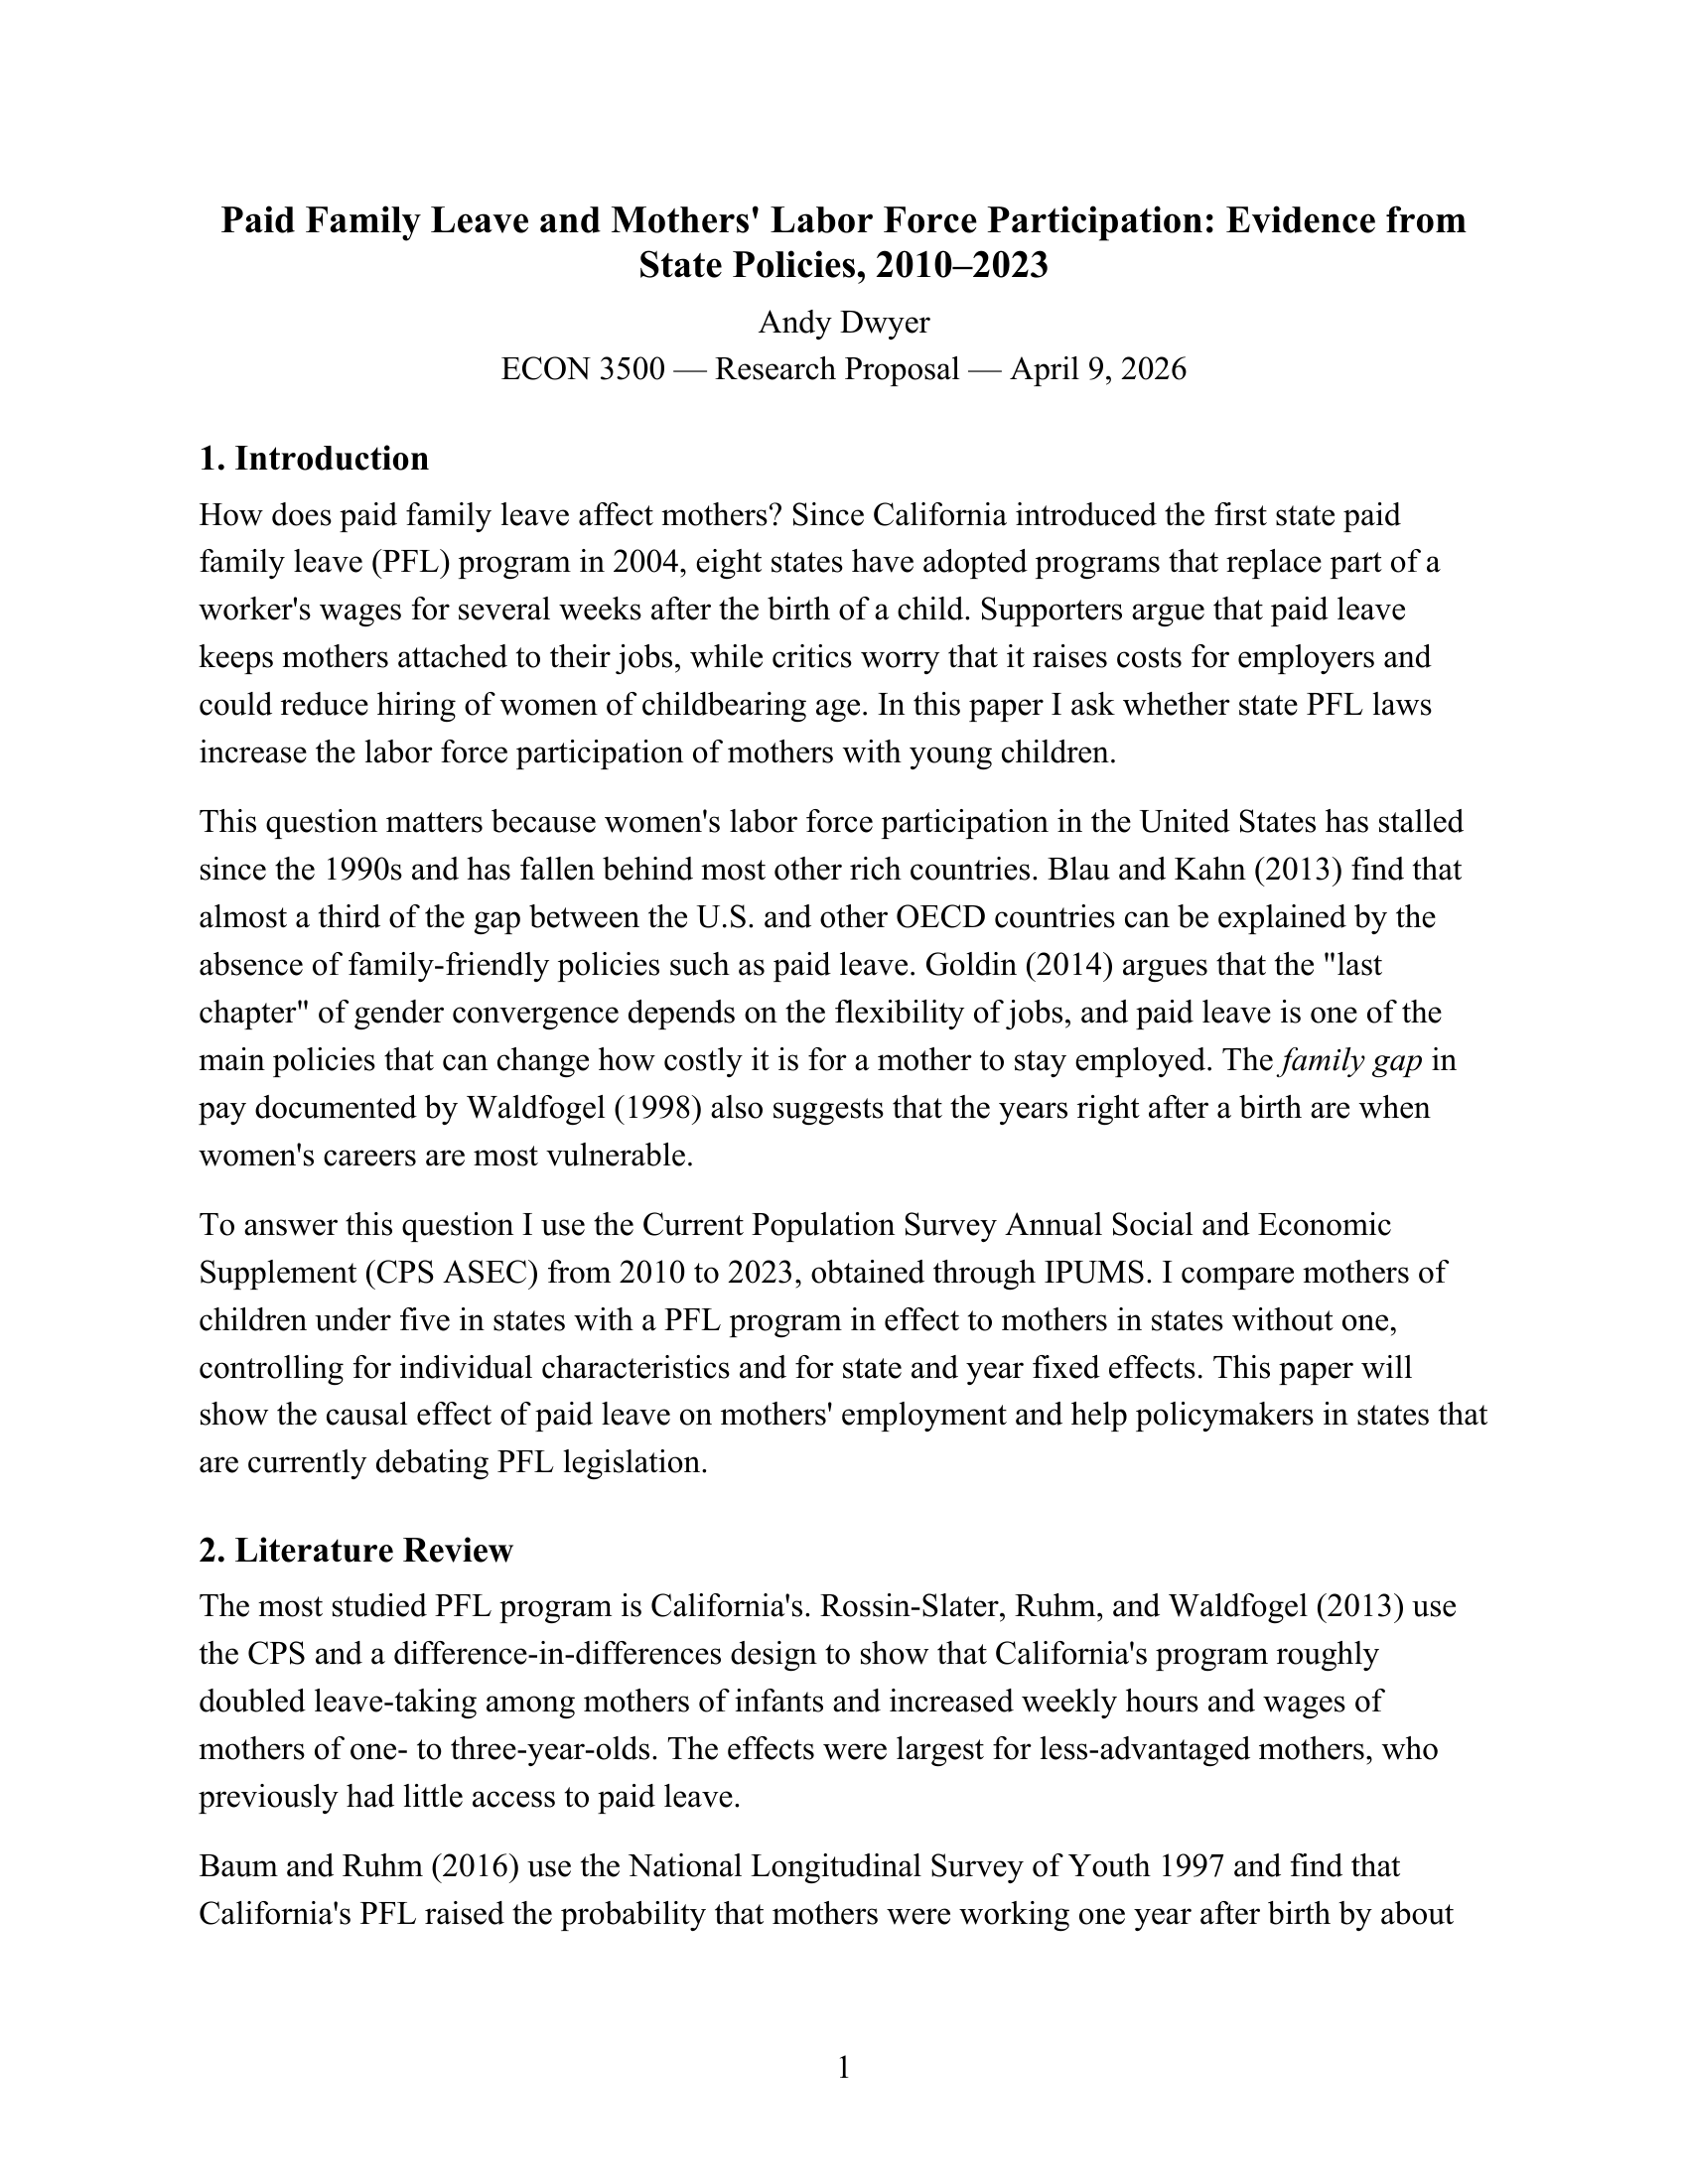
\includegraphics[width=\textwidth, height=0.76\textheight, keepaspectratio]{fake_proposal_p1}
\end{center}
\end{column}
\begin{column}{0.56\textwidth}
\begin{tcolorbox}[keybox, title={\faFlask\quad Why fake}, top=2pt, bottom=2pt]
\scriptsize
\begin{itemize}\setlength{\itemsep}{3pt}
  \item I can't put a real student's paper on this screen --- so I wrote one. Fictional author, fictional numbers, real citations, a topic unlike anything my S26 class turned in.
  \item \textbf{13 flaws planted on purpose}, each mapped to a rubric line: a lit review that summarizes instead of synthesizes, a working paper counted as peer-reviewed, ``this will \emph{prove}\,'' where it should hedge, a table with no group split, no clustering mentioned.
  \item \textbf{Answer key written first}, before any grader saw it. Target: \textbf{28.5/38} --- deliberately mid, because that's where graders actually differ. (Real class: median 31.25.)
\end{itemize}
\end{tcolorbox}
\vskip3pt
\begin{tcolorbox}[accentbox, top=1pt, bottom=1pt]
\scriptsize A grader you can't score is a grader you're trusting on vibes. This is the cheapest way I know to score one.
\end{tcolorbox}
\end{column}
\end{columns}
\end{frame}

%% ====== SLIDE: FOUR PASSES, ONE COMMAND ======
\begin{frame}{How it actually runs --- four passes, one command}
\vskip-4pt
\begin{columns}[T]
\begin{column}{0.40\textwidth}
\begin{center}
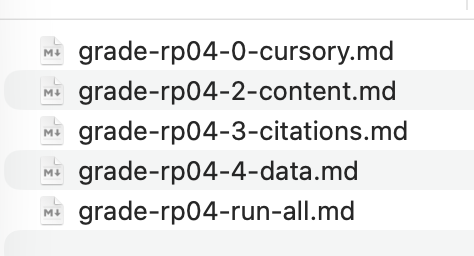
\includegraphics[width=0.95\textwidth, keepaspectratio]{rp04_prompts}
\end{center}
\vskip4pt
\begin{tcolorbox}[pipelinebox, title={\faTerminal\quad The fifth one is the whole trick}, top=2pt, bottom=2pt]
\scriptsize
\texttt{run-all} doesn't grade. It launches the other four \textbf{in parallel}, then adds up each student's criterion scores and checks they match the reported total. I run one file.
\end{tcolorbox}
\end{column}
\begin{column}{0.58\textwidth}
\begin{tcolorbox}[keybox, title={\faSitemap\quad One job each}, top=2pt, bottom=2pt]
\scriptsize
\begin{itemize}\setlength{\itemsep}{2.5pt}
  \item \textbf{cursory} --- an overview pass. Skim all 21 first, list the edge cases, write the rules \emph{before} anyone is graded.
  \item \textbf{content} --- the assignment and the rubric. The 38 points, and the feedback the student actually reads.
  \item \textbf{citations} --- a deliberately mechanical check: do these sources exist, are they peer-reviewed, do the counts hold? \emph{(I care about this more than I can fully justify.)}
  \item \textbf{data} --- will the data do what they say it will? Are the summary stats internally consistent? Does the specification match the data described?
\end{itemize}
\end{tcolorbox}
\vskip3pt
\begin{tcolorbox}[accentbox, top=2pt, bottom=2pt]
\scriptsize \textbf{Context I hand them:} the assignment description, \emph{and} my own feedback and grades on the two earlier assignments --- which is what lets the feedback say ``you did follow up on the concern I raised in February.''
\end{tcolorbox}
\end{column}
\end{columns}
\vskip2pt
\begin{tcolorbox}[coralbox, top=1pt, bottom=1pt]
\centering\scriptsize For 21 submissions, I'm honestly not sure it was \emph{faster}. It was more \textbf{consistent} --- and that's the part I couldn't do by hand at 11pm.
\end{tcolorbox}
\end{frame}

%% ====== SLIDE: FOUR GRADERS, ONE PROPOSAL ======
\begin{frame}{Four graders, one proposal}
\vskip-8pt
{\footnotesize A fake ECON 3500 proposal with 13 planted flaws. My real Spring 2026 grading prompt. Target: 28.5/38.\par}
\vskip2pt
\begin{columns}[T]
\begin{column}{0.54\textwidth}
{\scriptsize
\setlength{\tabcolsep}{3pt}
\renewcommand{\arraystretch}{1.05}
\begin{tabular}{>{\raggedright\arraybackslash}m{2.35cm} c c c c c}
\rowcolor{SlateTeal}
\textcolor{white}{\textbf{Component (pts)}} & \textcolor{white}{\textbf{Target}} & \textcolor{white}{\textbf{Copilot}} & \textcolor{white}{\textbf{Claude}} & \textcolor{white}{\textbf{Sonnet}} & \textcolor{white}{\textbf{Codex}} \\
\rowcolor{PaleSage} Introduction (6) & 4.5 & 6 & 6 & 6 & 6 \\
\rowcolor{white}    Literature (4) & 2 & 3 & \textbf{2} & 3 & \textbf{2} \\
\rowcolor{PaleSage} Data + table (6) & 5 & 6 & \textbf{5} & 6 & \textbf{5} \\
\rowcolor{white}    Empirical (10) & 7 & 7.5 & 8 & 8 & 7.5 \\
\rowcolor{PaleSage} Threats (2) & 1.5 & 2 & 2 & 2 & 2 \\
\rowcolor{white}    Presentation (10) & 8.5 & 9.5 & 9.5 & 9.5 & 9.5 \\
\rowcolor{LightGold} \textbf{Total (38)} & \textbf{28.5} & \textbf{34} & \textbf{32.5} & \textbf{34.5} & \textbf{32} \\
\rowcolor{white}    Flaws deducted (of 13) & --- & 4 & 6 & 3 & 6 \\
\rowcolor{PaleSage} Flaws invented & --- & 0 & 0 & 0 & 0 \\
\end{tabular}
}
\vskip4pt
{\scriptsize\color{CoolGray} Copilot with my NetID. Claude and Sonnet as fresh agents. Codex by hand.\par}
\end{column}
\begin{column}{0.44\textwidth}
\begin{tcolorbox}[keybox, title={\faSearch\quad What happened}, top=2pt, bottom=2pt]
\small
\begin{itemize}\setlength{\itemsep}{3pt}
  \item Everyone drifted up --- on the judgment criteria.
  \item The checks held: both overclaims, the missing reference, the source count.
  \item Nobody hallucinated. Sonnet noticed nine flaws and deducted for three.
\end{itemize}
\end{tcolorbox}
\vskip4pt
\begin{tcolorbox}[accentbox, top=2pt, bottom=2pt]
\small \textbf{Read the notes, not the numbers.}
\end{tcolorbox}
\end{column}
\end{columns}
\end{frame}

%% ====== SLIDE: WHAT THE FEEDBACK READ LIKE ======
\begin{frame}{What the feedback read like}
\vskip-6pt
{\footnotesize Each grader also wrote the student feedback my prompt asks for. Compared to one I wrote in April.\par}
\vskip3pt
\begin{columns}[T]
\begin{column}{0.49\textwidth}
\begin{tcolorbox}[keybox, title={\faTools\quad Most useful}, top=2pt, bottom=2pt]
\small
\begin{itemize}\setlength{\itemsep}{3pt}
  \item \textbf{Codex.} My length. Handed the student the sentence to use instead of ``prove.''
  \item \textbf{Claude.} Most complete. Three times my length.
  \item \textbf{Sonnet.} Fine. Called four summaries ``genuinely good synthesis.''
\end{itemize}
\end{tcolorbox}
\end{column}
\begin{column}{0.49\textwidth}
\begin{tcolorbox}[keybox, title={\faComment\quad Closest to my voice}, top=2pt, bottom=2pt]
\small
\begin{itemize}\setlength{\itemsep}{3pt}
  \item \textbf{Claude} got the structure: the name, the quoted sentences, the headers.
  \item \textbf{Codex} got the economy.
  \item \textbf{Nobody} got the pivot. No ``That said,'' no closing on the positive.
\end{itemize}
\end{tcolorbox}
\end{column}
\end{columns}
\vskip6pt
\begin{tcolorbox}[accentbox, halign=center, top=3pt, bottom=3pt]
\small The substance is theirs. The voice is a five-minute edit.
\end{tcolorbox}
\end{frame}

%% ====== SLIDE: THE PIPELINE ======
\begin{frame}{What I do at scale --- same rubric, different plumbing}
\vskip-4pt
\begin{center}
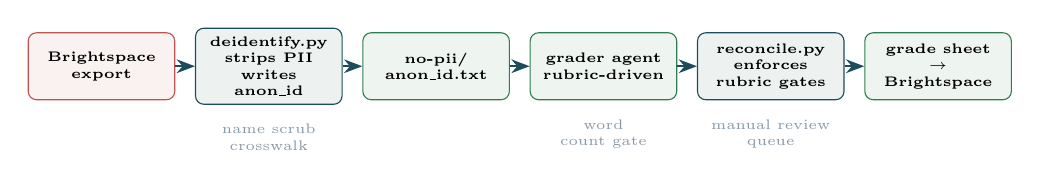
\begin{tikzpicture}[
  node distance=0.4cm and 0.25cm,
  box/.style={rectangle, rounded corners=3pt, draw=SlateTeal, fill=PaleSage,
    text width=1.65cm, align=center, font=\tiny\bfseries, minimum height=0.85cm,
    inner sep=3pt},
  piibox/.style={rectangle, rounded corners=3pt, draw=SoftCoral, fill=SoftCoral!8,
    text width=1.65cm, align=center, font=\tiny\bfseries, minimum height=0.85cm,
    inner sep=3pt},
  safenode/.style={rectangle, rounded corners=3pt, draw=GoGreen, fill=GoGreen!8,
    text width=1.65cm, align=center, font=\tiny\bfseries, minimum height=0.85cm,
    inner sep=3pt},
  arr/.style={-Stealth, thick, color=SlateTeal},
  label/.style={font=\tiny\color{CoolGray}, align=center, text width=1.65cm}
]
  \node[piibox] (bs)   {Brightspace\\export};
  \node[box, right=of bs] (deid)  {deidentify.py\\strips PII\\writes anon\_id};
  \node[safenode, right=of deid] (nopii) {no-pii/\\anon\_id.txt};
  \node[safenode, right=of nopii] (agent) {grader agent\\rubric-driven};
  \node[box, right=of agent] (rec)  {reconcile.py\\enforces\\rubric gates};
  \node[safenode, right=of rec] (out)  {grade sheet\\$\rightarrow$ Brightspace};

  \draw[arr] (bs) -- (deid);
  \draw[arr] (deid) -- (nopii);
  \draw[arr] (nopii) -- (agent);
  \draw[arr] (agent) -- (rec);
  \draw[arr] (rec) -- (out);

  \node[label, below=0.12cm of deid] {name scrub\\crosswalk};
  \node[label, below=0.12cm of agent] {word count gate};
  \node[label, below=0.12cm of rec]  {manual review\\queue};
\end{tikzpicture}
\end{center}
\vskip3pt
\begin{tcolorbox}[accentbox, top=2pt, bottom=2pt]
\centering\small \textbf{At no point does the AI see a name} --- which is what lets me use whatever model follows the rubric best.
\end{tcolorbox}
\vskip2pt
\begin{columns}[T]
\begin{column}{0.48\textwidth}
\begin{tcolorbox}[pipelinebox, title={\faUsers\quad Why the plumbing}]
\scriptsize
De-identify once $\rightarrow$ two graders (fair + strict) + an auditor $\rightarrow$ deterministic reconciliation $\rightarrow$ only disagreements reach me. The agent wrote the scripts; I described the rubric and the export.
\end{tcolorbox}
\end{column}
\begin{column}{0.48\textwidth}
\begin{tcolorbox}[pipelinebox, title={\faBalanceScale\quad When it's worth it}]
\scriptsize
Research papers, 18 criteria, 17 students: yes. Three-question completion essays: Copilot and a good rubric are enough. The rubric is the same file either way.
\end{tcolorbox}
\end{column}
\end{columns}
\end{frame}

%% ====== SLIDE: SHOULD AI BE GRADING AT ALL? ======
\begin{frame}{``Should AI be grading at all?''}
\vskip-2pt
{\small A fair question, and one a faculty attendee put to us bluntly at the June webinar. My honest answer, in three parts:}
\vskip3pt
\begin{columns}[T]
\begin{column}{0.32\textwidth}
\begin{tcolorbox}[keybox, title={1. What I let it grade}, top=2pt, bottom=2pt]
\footnotesize \textbf{Rubric-gated completion work} --- did they answer all six questions, at length, thoughtfully. Not the term paper. Not anything where the grade \emph{is} the feedback.
\end{tcolorbox}
\end{column}
\begin{column}{0.32\textwidth}
\begin{tcolorbox}[keybox, title={2. It's an RA, not a referee}, top=2pt, bottom=2pt]
\footnotesize Same contract as a TA: it does a first pass, I check what it flags and spot-check what it didn't, and \textbf{the errors are mine either way}. Nothing about that changed.
\end{tcolorbox}
\end{column}
\begin{column}{0.32\textwidth}
\begin{tcolorbox}[keybox, title={3. Consistency is a process}, top=2pt, bottom=2pt]
\footnotesize My own first pass under-scored 11 of 17 papers; the second pass caught it. The comparison isn't AI vs.\ a perfect grader --- it's AI-plus-review vs.\ me, essay 43 of 60, at 10pm.
\end{tcolorbox}
\end{column}
\end{columns}
\vskip5pt
\begin{tcolorbox}[accentbox, top=3pt, bottom=3pt]
\small What I don't have a settled answer on: \textbf{disclosure.} Do we tell students? What do we tell them? I'd genuinely like to know where this room lands.
\end{tcolorbox}
\end{frame}

%% ============================================================
%% WHERE THIS COULD GO + HANDOFF (~3 min)
%% ============================================================

\begin{frame}{Where this could go for us}
\vskip2pt
\begin{columns}[T]
\begin{column}{0.48\textwidth}
\begin{tcolorbox}[keybox, title={\faCalendar\quad What Erkmen and I are planning}]
\small
\begin{itemize}\setlength{\itemsep}{3pt}
  \item \textbf{November:} start concrete planning for an AI-assisted grading setup that others in the department could pick up --- target early 2027
  \item \textbf{Next TwA webinar:} deferred to November, when we'll have new material
  \item Happy to sit down with anyone one-on-one --- setup takes an afternoon
\end{itemize}
\end{tcolorbox}
\end{column}
\begin{column}{0.48\textwidth}
\begin{tcolorbox}[accentbox, title={\faComments\quad Three things worth talking about}, fonttitle=\bfseries\small, coltitle=DeepCharcoal, colbacktitle=LightGold!80]
\small
\begin{enumerate}\setlength{\itemsep}{3pt}
  \item \textbf{Disclosure norms.} What do we say to students about our own use?
  \item \textbf{Which of our courses} have the mechanical-grading problem where this actually helps?
  \item \textbf{What would make it easy to try} --- a shared setup, a template, a lunch?
\end{enumerate}
\end{tcolorbox}
\vskip4pt
\begin{center}\begin{tcolorbox}[accentbox, halign=center, width=6.2cm, top=2pt, bottom=2pt]
\small\bfseries thinkingwithagents.github.io
\end{tcolorbox}\end{center}
\end{column}
\end{columns}
\end{frame}

{
\setbeamertemplate{footline}{}
\setbeamercolor{background canvas}{bg=SlateTeal}
\begin{frame}[plain, noframenumbering]
\centering\vfill
{\fontsize{20}{26}\bfseries\selectfont\color{white} Over to Erkmen}\\[8pt]
{\color{UVMGold}\rule{6cm}{0.8pt}}\\[8pt]
\begin{tcolorbox}[accentbox, width=11cm, top=4pt, bottom=4pt]
\centering\small
\textbf{My half in one line:} it makes a better lecture feasible and a good-enough one cheap $\cdot$ know the UVM rule $\cdot$ write a rubric with gates and checks $\cdot$ let the agent do the checks $\cdot$ you keep the judgment.
\end{tcolorbox}
\vskip10pt
{\normalsize\color{PaleSage} Erkmen: what the evidence says, how others are using it, and a live dashboard.}
\vfill
\end{frame}
}

\end{document}
